\documentclass{article}
\usepackage{graphicx}
\usepackage{amsmath}
\usepackage{pgfplots}
\usepackage{ragged2e}
\pgfplotsset{compat=1.18}
\usepackage{float} % Add this line

\begin{document}

\section*{1) Enunciado del Problema}

Un chico de \textbf{21 años}  se dispone a circular por el carril bici del Paralelo de Barcelona con un patinete eléctrico. El patinete tiene un ordenador interno para conocer en todo momento la velocidad y el estado de la batería. La autonomía que permite la batería es de \textbf{25 km}, la velocidad máxima es de \textbf{25 km/h} y tiene 3 tipos de sistemas de frenos. El chico está en un semáforo parado, sube al patinete inicialmente en reposo y cuando el semáforo se pone en verde, es capaz de acelerar de \textbf{0 km/h} a \textbf{15,3 km/h} en \textbf{1,7} segundos en un tramo sin fricción.

% section 1a ----------------------------------------------------------------------------------------------------

\section*{1a) Conversiones de Unidades S.I}

\begin{itemize}
    \item Edad: \[
21 \, \text{años} = 21 \times \frac{365.25 \, \text{días}}{1 \, \text{año}} \times \frac{24 \, \text{horas}}{1 \, \text{día}} \times \frac{60 \, \text{minutos}}{1 \, \text{hora}} \times \frac{60 \, \text{segundos}}{1 \, \text{minuto}} = \boxed{662709600\, \text{s}}
\]
    \item Autonomía: \(25 \, \text{km} = 25 \text{km}\times \frac{1000 \text{m}}{1 \text{km}}{} \, = \boxed{25\,000 \, \text{m}}\)
    \item \(V_{\text{max}}: 25 \, \text{km/h} = 25\, \text{km/h} \times \frac{1000\,\text{m}}{1\,\text{km}} \times \frac{1\,\text{h}}{3600\,\text{s}} \, \approx \boxed{6,94 \, \text{m/s}} \)
    \item \(V_0: 0 \, \text{km/h} = \boxed{0 \, \text{m/s}}\)
    \item \(V: 15,3 \, \text{km/h} = 15,3\, \text{km/h} \times \frac{1000\,\text{m}}{1\,\text{km}} \times \frac{1\,\text{h}}{3600\,\text{s}} \, = \boxed{4,25 \, \text{m/s}} \)
    \item Tiempo: \(1,7 \, \text{segundos} = \boxed{1.7 \, \text{s}}\)
\end{itemize}

% section 1b ----------------------------------------------------------------------------------------------------

\section*{1b) Cálculo de la aceleración media}

Para calcular la aceleración media (\(a\)) que experimenta el patinete, podemos utilizar la fórmula de la aceleración media, que se da por:

\[
a = \frac{\Delta_V}{\Delta_t}
\]

Sustituyendo los valores:

\begin{itemize}
    \item \(V = 4.25 \, \text{m/s}\) (velocidad final después de la aceleración),
    \item \(V_0 = 0 \, \text{m/s}\) (inicialmente en reposo),
    \item \(t = 1.7 \, \text{s}\) (tiempo final de la aceleracion),
    \item \(t_0 = 0 \, \text{s}\) (tiempo inicial, en que el patinete empieza a acelerar),

\end{itemize}

Ahora podemos calcular:

\[
a = \frac{4.25 \, \text{m/s} - 0 \, \text{m/s}}{1.7 - 0 \, \text{s}} = \frac{4.25 \, \text{m/s}}{1.7 \, \text{s}} = \boxed {2.5 \, \text{m/s}^2}
\]

\subsection*{Justificación del Signo del Resultado}

El signo de la aceleración es positivo, lo que indica que la patineta está acelerando. Una aceleración positiva significa que la velocidad del patinete está aumentando, lo que es coherente con el hecho de que el patinete comenzó desde el estado de inactividad y aumentó su velocidad al acelerar. Por lo tanto, la justificación del signo del resultado es que el patinete está en movimiento acelerado, saliendo del estado de reposo y aumentando su velocidad a lo largo del tiempo.

% section 1c ----------------------------------------------------------------------------------------------------

\section*{1c) Cálculo de la distancia recorrida por el patinete durante el tiempo de aceleración}

Para calcular la distancia recorrida por el patinete durante el tiempo en que estuvo acelerando, utilizamos la ecuación del movimiento uniformemente acelerado:

\[
S(t) = S_0 + V_0 t + \frac{1}{2} a t^2
\]

En este caso, estamos interesados en la variación de la posición (\(\Delta S\)), que se calcula como:

\[
\Delta S = S(t) - S(0)
\]

Donde:
\begin{itemize}
    \item \(\Delta S\) es la distancia recorrida,
    \item \(S(0)\) = 0 m
    \item \(V_0\) = 0 m/s (velocidad inicial, en reposo),
    \item \(t\) es el tiempo que el patinete estuvo acelerando (\(1,7 \, \text{s}\)),
    \item \(a\) es la aceleración (\(2,5 \, \text{m/s}^2\)).
\end{itemize}

Sustituyendo los valores en la ecuación:

\[
    S(t) = \frac{1}{2} a t^2
\]

\[
    \Delta S = \frac{1}{2} \times 2.5 \, \frac{\text{m}}{\text{s}^2} \times (1.7 \, \text{s})^2 \approx \boxed{3.61 \, \text{m}}
\]

% section 1d ----------------------------------------------------------------------------------------------------

\section*{1d) Aceleración de frenado}

Para calcular la aceleración de frenado (\(a_{\text{frenado}}\)) que experimenta el patinete al detenerse, podemos utilizar la ecuación de Torricelli dada por:

\[
V^2 = V_0^2 + 2 a_{\text{frenado}} S
\]

% subsection 1.1d -!-!-!-!-!-!-!-!-!-!-!-!-!-!-!-!-!-!-!-!-!-!-!-!-!-!-!-!-!-!-!-!-!-!-!-!-!-!-!-!-!-!-!-!-!-!-!-

\subsection*{1.1d) Demostración de la fórmula \( V^2 = V_0^2 + 2ad \)}
Partimos de las definiciones de aceleración y de las ecuaciones del movimiento.

\[
a = \frac{V - V_0}{t}
\]

\[
d = V_0 t + \frac{1}{2} a t^2
\]

1. Reordenando la ecuación de la aceleración:
\[
V - V_0 = a t \implies t = \frac{V - V_0}{a}
\]

2. Sustituyendo \(t\) en la fórmula de la distancia:
\[
d = V_0 t + \frac{1}{2} a t^2
\]
\[
d = V_0 \left(\frac{V - V_0}{a}\right) + \frac{1}{2} a \left(\frac{V - V_0}{a}\right)^2
\]

3. Desarollando la ecuación:
\[
d = \frac{V_0 (V - V_0)}{a} + \frac{(V - V_0)^2}{2a}
\]

4. Multiplicando toda la ecuación por \(2a\) para eliminar los denominadores:
\[
2ad = 2V_0 (V - V_0) + (V - V_0)^2
\]
\[
2ad = (2V_0 V - 2V_0^2) + (V^2 - 2V_0 V_0 - V_0^2) 
\]

5. Simplificando la ecuación:
\[
2ad = V^2 + (2V_0^2 - V_0^2) 
\]

\[
2ad = V^2 - V_0^2
\]

\[
\boxed{ V^2=     V_0^2 + 2a\Delta S }
\]
`'
% subsection 1.2d -!-!-!-!-!-!-!-!-!-!-!-!-!-!-!-!-!-!-!-!-!-!-!-!-!-!-!-!-!-!-!-!-!-!-!-!-!-!-!-!-!-!-!-!-!-!-!-

\subsection*{1.2d) Resolución del cálculo de la aceleración de frenado}

Para calcular la aceleración de frenado del patinete, utilizamos la ecuación de Torricelli que acabamos de demostrar:

\[
V^2 = V_0^2 + 2ad
\]

Donde:
\begin{itemize}
    \item \(V\) es la velocidad final (\(0 \, \text{m/s}\), ya que el patinete se detiene),
    \item \(V_0\) es la velocidad inicial (\(19,5 \, \text{km/h}\)),
    \item \(a\) es la aceleración (que deseamos calcular),
    \item \(d\) es la distancia recorrida durante la frenada (\(11 \, \text{m}\)).
\end{itemize}

Primero, convertimos la velocidad inicial \(V_0\) de km/h a m/s:

\[
V_0 = 19,5 \, \text{km/h} = 19,5 \times \frac{1000 \, \text{m}}{3600 \, \text{s}} \approx 5,416 \, \text{m/s}
\]

\justify
A partir de aquí, podemos ignorar las unidades de medida, ya que todas las cantidades están en el sistema internacional. Por lo tanto, la aceleración que calcularemos también se expresará en este sistema. Al sustituir los valores en la fórmula, obtenemos:

\[
0 = 5,416^2 + 2a*11
\]

\[
0 = 29,340 + 22a
\]

Despejamos \(a\):

\[
22a = -29,340 \implies a = \frac{-29,34}{22} \approx \boxed{-1,333 \, \text{m/s}^2}
\]

\subsection*{Justificación del signo del resultado}

El signo negativo de la aceleración indica que el patinete está desacelerando. Esto es coherente con el hecho de que se está deteniendo. Una aceleración negativa indica que la velocidad del patinete está disminuyendo, lo que corresponde a un proceso de frenado.

% section 1e ----------------------------------------------------------------------------------------------------

\subsection*{1e) Cálculo del tiempo que ha tardado el patinete en el apartado 1d}


\begin{itemize}
    \item Velocidad inicial (\( V_0 \)): \( 19,5 \, \text{km/h} = 5,416 \, \text{m/s} \)
    \item Velocidad final (\( V \)): \( 0 \, \text{m/s} \)
    \item Aceleración (\( a \)): \( -1,333 \, \text{m/s}^2 \)
\end{itemize}

Usamos la fórmula:

\[
V = V_0 + at
\]

Sustituyendo los valores:

\[
0 = 5,416 \, \text{m/s} + (-1,333 \, \text{m/s}^2) t 
\]

\justify
A partir de aquí, podemos ignorar las unidades de medida, ya que todas las cantidades están en el sistema internacional. Por lo tanto, lo que calcularemos también se expresará en este sistema. Aislando \( t\), obtendremos:

\[
1,333 \, t = 5,416 
\]
\[
t = \frac{5,416}{1,333} \approx \boxed{4,06 \, \text{s}}
\]

\justify
Por lo tanto, el tiempo que el patinete tardó en detenerse durante el frenado es aproximadamente \( 4,06 \) segundos.

\section*{2) Enunciado del Problema}


\begin{figure}[h] % 'h' significa aquí; también puedes usar 't' para arriba, 'b' para abajo
    \centering
    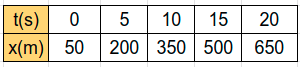
\includegraphics[width=0.7\textwidth]{tabla.png} % Cambia a tu nombre de archivo
    \caption{La tabla anterior muestra la posición de un coche en función del tiempo en un movimiento rectilíneo.
    }
    \label{fig:tabla}
\end{figure}\

% section 2a ----------------------------------------------------------------------------------------------------

\section*{2a) Representación gráfica de la posición}

\begin{figure}[h] % 'h' significa aquí; también puedes usar 't' para arriba, 'b' para abajo
    \centering
    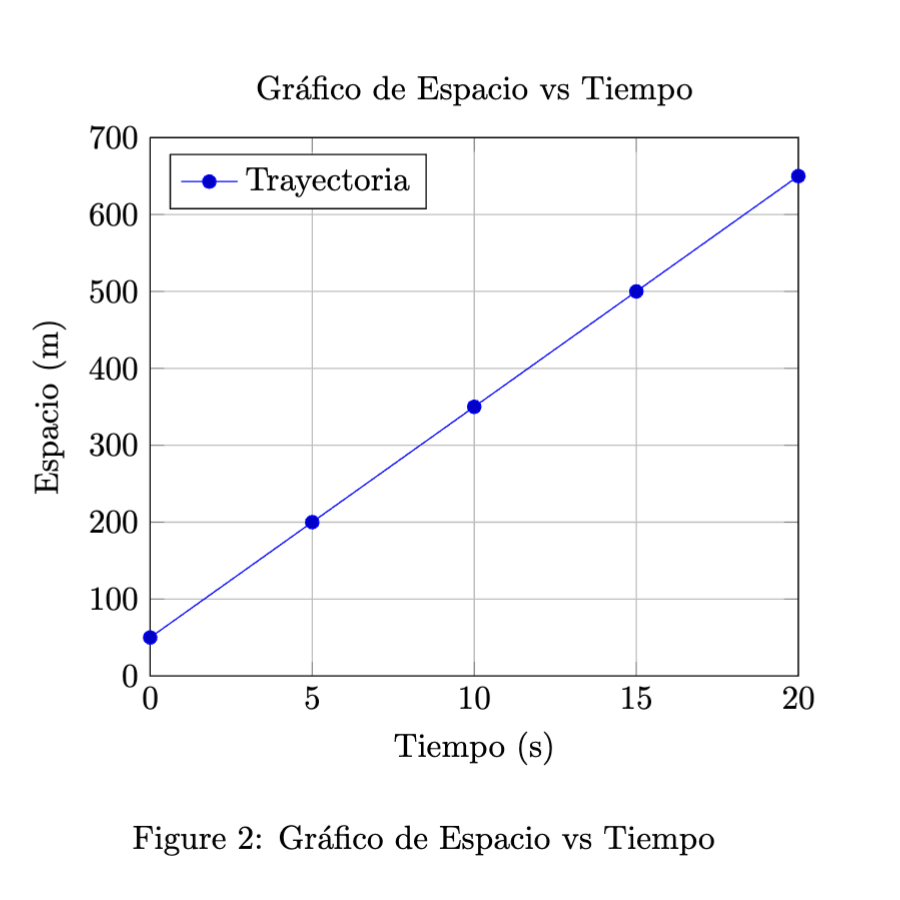
\includegraphics[width=0.7\textwidth]{grafico.png} % Cambia a tu nombre de archivo
    \caption{La gráfica anterior muestra la posición de un coche en función del tiempo en un movimiento rectilíneo.
    }
    \label{fig:grafico}
\end{figure}\

% section 2b ----------------------------------------------------------------------------------------------------

\section*{2b) Cálculo de la velocidad media}

Para calcular la velocidad media (\(v_m\)), utilizamos:

\[
v_m = \frac{\Delta S}{\Delta t}
\]

1. Desplazamiento (\(\Delta S\)):
   \[
   \Delta S = S_{final} - S_{inicial} = 650 \, \text{m} - 50 \, \text{m} = 600 \, \text{m}
   \]

2. Intervalo de tiempo (\(\Delta t\)):
   \[
   \Delta t = t_{final} - t_{inicial} = 20 \, \text{s} - 0 \, \text{s} = 20 \, \text{s}
   \]

3. Cálculo de la velocidad media m/s:
\[
v_m = \frac{600 \, \text{m}}{20 \, \text{s}} = \boxed{30 \, \text{m/s}}
\]

Ahora, para convertir a km/h:
\[
v_m = 30 \, \text{m/s} \times \frac{3600 \, \text{s}}{1000 \, \text{m}} = \boxed{108 \, \text{km/h}}
\]

Por lo tanto, la velocidad media es:

\begin{itemize}
    \item \(v_m = 30 \, \text{m/s}\)
    \item \(v_m = 108 \, \text{km/h}\)
\end{itemize}

% section 2c ----------------------------------------------------------------------------------------------------

\section*{2c) Tipo de Movimiento}

\subsection*{Análisis de la velocidad media}

La velocidad media calculada es de \(30 \, \text{m/s}\). Observando los datos de posición:

\begin{itemize}
    \item Entre \(t = 0\) y \(t = 5\) segundos, el coche se desplaza de \(50 \, \text{m}\) a \(200 \, \text{m}\) (desplazamiento de \(150 \, \text{m}\)).
    \item Entre \(t = 5\) y \(t = 10\) segundos, va de \(200 \, \text{m}\) a \(350 \, \text{m}\) (también \(150 \, \text{m}\)).
    \item Entre \(t = 10\) y \(t = 15\) segundos, se mueve de \(350 \, \text{m}\) a \(500 \, \text{m}\) (otra vez \(150 \, \text{m}\)).
    \item Finalmente, entre \(t = 15\) y \(t = 20\) segundos, va de \(500 \, \text{m}\) a \(650 \, \text{m}\) (nuevamente \(150 \, \text{m}\)).
\end{itemize}

\subsection*{Explicación:}

Aunque el coche parece tener un movimiento uniforme entre los puntos observados, no se puede garantizar que sea así, ya que los datos son puntos aislados. La representación lineal solicitada en el ejercicio 1a) no implica un movimiento constante.
Pero creo que para los fines de este ejercicio, la respuesta esperada sería: "Sí, es MRU."

\begin{itemize}
    \item Tipo de Movimiento: \textbf{M.R.U} (Movimiento Recto Uniforme)
    \item Razón: La variación de espacio-tiempo es uniforme. Por lo tanto, la velocidad media es constante en cada intervalo de tiempo, lo que significa que no hay aceleración (\(a = 0 \, \text{m/s}^2\)) y, por lo tanto, \textbf{el movimiento es uniforme y no variado}, porque no tiene aceleración. 
\end{itemize}

% section 2d ----------------------------------------------------------------------------------------------------

\section*{2d) Cálculo de la posición del coche a los 90 segundos}

Dado que el coche tiene una posición inicial de \(S_0 = 50 \, \text{m}\) y una velocidad constante de \(V_0 = 30 \, \text{m/s}\), podemos utilizar la fórmula de la posición en función del tiempo:

\[
S(t) = S_0 + V_0 \cdot t
\]

Sustituimos \(t = 90 \, \text{segundos}\):

\[
S(90) = 50 \, \text{m} + 30 \, \text{m/s} \times 90 \, \text{s}
\]

Calculando:

\[
S(90) = 50 + 2700 = \boxed{2750 \, \text{m}}
\]

% section 2e ----------------------------------------------------------------------------------------------------

\section*{2e) Cálculo de el desplazamiento del coche}

Dado que \( S(90) = 2750 \, \text{m} \) y \( S_0 = 50 \, \text{m} \), podemos calcular el desplazamiento \(\Delta S\):

\[
\Delta S = S - S_0 = 2750 \, \text{m} - 50 \, \text{m} = \boxed{2700 \, \text{m}}
\]

\justify
Por lo tanto, el coche se ha desplazado \( 2700 \, \text{m} \) desde su posición inicial.

\end{document}